\documentclass[a4paper,12pt]{article}
\usepackage{latexsym}
\usepackage{graphicx}
\usepackage{epsfig}
\usepackage{float}
\usepackage{natbib}
\usepackage{listings}
\usepackage{amsmath}
\usepackage{gensymb}
\graphicspath{{./}}
\DeclareGraphicsExtensions{.jpg}
\author{Howard Kinsman}
\title{Cosmology Tutorial 10}
\begin{document}
\maketitle
\section{}
The Sloan Digital Sky Survey (SDSS) saw first light in 1998 and its scope has changed over the years. Current surveys (2014-2020) include:
\newline
eBOSS - Extended Baryon Oscillation Spectroscopic Survey - which is a spectroscopic survey of galaxies and quasars up to redshift z=3.
\newline
APOGEE-2 - APO Galaxy Evolution Experiment - infrared spectroscopic suvery of Milky Way.
\newline
MaNGA - Obtaining spectra of entire face of targetted local galaxies.

The general goals of SDSS are to use highly efficient instruments and software to create high quality surveys and public datasets and to make use
of international collaboration.
\section{} 
The ALFALFA survey is a HI survey and so maps extraglactic HI sources and then tries to map these to optical sources. It differs from other surveys in that
it detects HI line sources.

Figure 1 shows a histogram of the HI flux density, and shows the total survey data together with flux limited and volume limited samples. I chose 100 Jy  km/s
as the flux limit.
\begin{figure}[H]
\centering
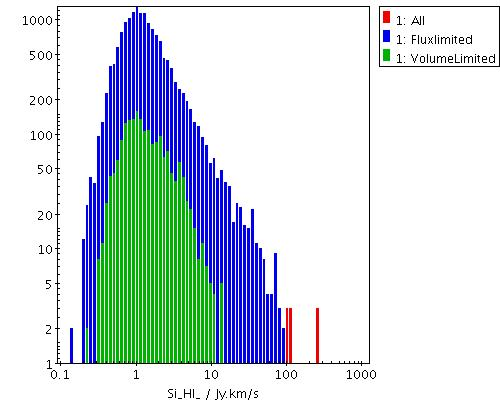
\includegraphics[width=.9\textwidth]{./SiH1.jpg}
\caption{}
\label{fig:1}
\end{figure}
Figure 2 shows mass plotted with distance and also shows the volume limited sample from 80 to 100 Mpc. I have to admit I was unsure of how to select a
volume limited sample and this step seems very arbitrary - so probably my lack of understanding.
\begin{figure}[H]
\centering
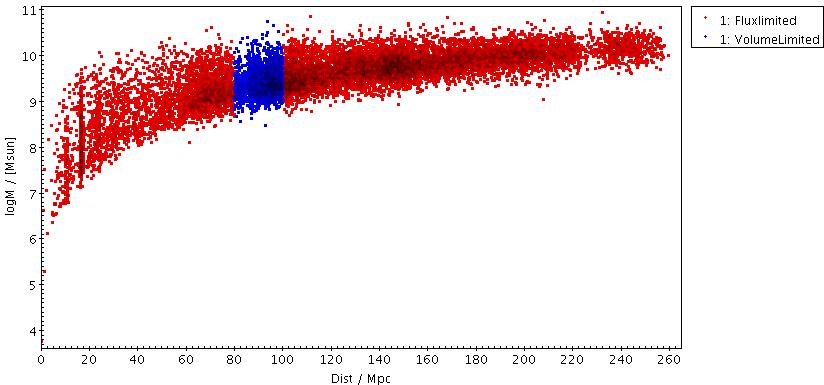
\includegraphics[width=.9\textwidth]{./MassDistance.jpg}
\caption{}
\label{fig:2}
\end{figure}
Figure 3 is a histogram of the mass from the volume limited sample and shows the mass function.
\begin{figure}[H]
\centering
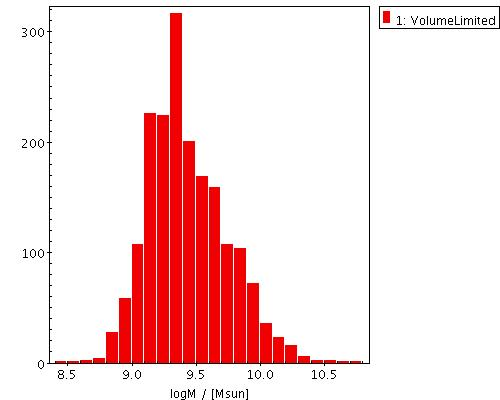
\includegraphics[width=.9\textwidth]{./MassFunction.jpg}
\caption{}
\label{fig:3}
\end{figure}
The survey area of ALFALFA was 6300 square degrees which is 1.92 steradians so,
\begin{flalign*}
& V=\frac{1}{3}\Omega\left[D(z_{max})^3-D(z_{min})^3\right] &\\
& = \frac{1}{3}\times1.92\times\left(100^3-80^3\right) &\\
& =312,320 Mpc^{-3}
\end{flalign*}
I think I was supposed to use comoving distance for the above calculation but don't know how to get from data given.
\section{}
I couldn't do question 3.
\section{}
\begin{flalign*}
& PSFR(z)=.015\frac{\left(1+z\right)^{2.7}}{1+\left[\left(1+z\right)/2.9\right]^{5.6}} &\\
& =.015\frac{4^{2.7}}{1+\left(4/2.9\right)^{5.6}} &\\
& =.0898M_{\odot}yr^{-1}Mpc^{-3}
\end{flalign*}
Comvoing volume is used in order to compare the SFR density of galaxies at different redshifts i.e. the expansion
of the universe needs to be accounted for.
\section{}
Passive galaxies tend to occupy virialised (high-density) clusters and so have higher velocity dispersions.
From Madgwick et al., 2003, The 2dF Galaxy Redshift Survey: galaxy clustering per spectral type.
\section{}
Solid line is CDM as it dominates.
\newline
Dashed line is baryonic matter as it shows the BAO peak at around 100 Mpc.
\newline
I don't know what the dotted line is - Neutrinos?
\section{}
An additional neutrino species would increase the horizon scale at the time of photon-baryobn decoupling.
This would lead to values of $H_0$ that are in agreement with other measurements i.e. the distance ladder
and inverse distance ladder would agree.
%\begin{thebibliography}{1}
%\end{thebibliography}
\end{document} 